\documentclass[crop,tikz]{standalone}
\usetikzlibrary{backgrounds}
\colorlet{blue}{cyan}
\tikzset{
  inverted/.style = {
    color=white,
    background rectangle/.style={fill},
    show background rectangle
  }
}

\usepackage[european]{circuitikz}

\begin{document}
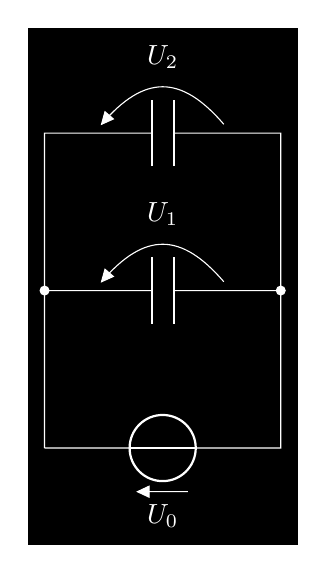
\begin{tikzpicture}[inverted,inverted]
  \draw (-1.5,0)
    to[V,v_<=$U_0$] ++(3,0)
    to[short,-*] ++(0,2)
    to[C,v=$U_1$] ++(-3,0)
    to[short,*-] ++(0,-2);
  \draw (1.5,2)
    to ++(0,2)
    to[C,v=$U_2$] ++(-3,0)
    to ++(0,-2);
\end{tikzpicture}
\end{document}
